\subsubsection{Server - OrderGateway}
\begin{figure}[H]
	\centering
%	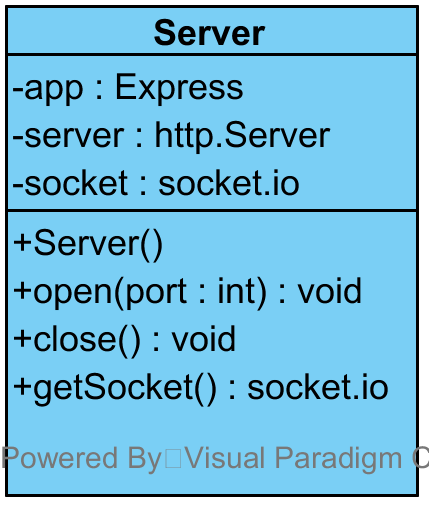
\includegraphics[width=15cm]{./diagrammi/demo/server.png}
	\caption{Componente OrderGateway}
\end{figure}
Il server è composto dall'OrderGateway, che ne è la base, dal package Order, che contiene le classi che rappresentano degli ordini, e da Menu, il quale fornisce e gestisce varie operazioni.

\setclass{BubbleAndEat::OrderGateway::Order}
\paragraph[::Order]{\class}\mbox{}\\ \label{\class}
\begin{figure}[H]
	\centering
%	\includegraphics[width=15cm]{./diagrammi/demo/order.png}
	\caption{Componente \class}
\end{figure}

Questo componente ha la funzione di rappresentare gli ordini.

\setclass{BubbleAndEat::OrderGateway::Order::Order}
\subparagraph[::Order]{\class}\mbox{}\\ \label{\class}
\begin{figure}[H]
	\centering
%	\includegraphics[width=15cm]{./diagrammi/demo/server/order/order.png}
	\caption{Classe \class}
\end{figure}
\textbf{Descrizione:}\\
Classe che rappresenta un singolo ordine.

\textbf{Utilizzo:}\\
Viene utilizzata per creare e effettuare operazioni sugli ordini.

%\textbf{Classi ereditate:}
%\begin{itemize}
%	\item \code{}.
%\end{itemize}
%
%\textbf{Sottoclassi:}
%\begin{itemize}
%	\item \coderef{}.
%\end{itemize}

\textbf{Attributi:}
\begin{itemize}
	\item \field{id: int}: numero identificativo dell'ordine;
	\item \field{client: Client}: cliente che ha effettuato l'ordine;
	\item \field{dishes: MenuItem[]}: lista dei piatti ordinati;
\end{itemize}

\textbf{Metodi:}
\begin{itemize}
	\item \method{process}
\end{itemize}

\setclass{BubbleAndEat::OrderGateway::OrderItem}
\subparagraph[::OrderItem]{\class}\mbox{}\\ \label{\class}
\begin{figure}[H]
	\centering
	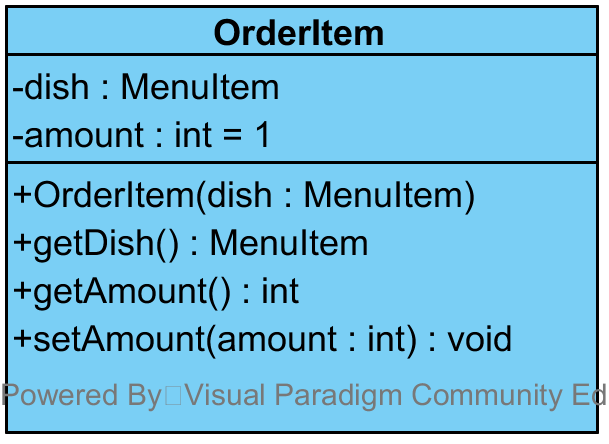
\includegraphics[width=7cm]{./diagrammi/demo/server/order/orderitem.png}
	\caption{Classe \class}
\end{figure}
\textbf{Descrizione:}\\
Classe che rappresenta una pietanza dell'ordine.

\textbf{Utilizzo:}\\
Viene utilizzata per memorizzare le quantità per ogni singolo piatto incluso nell'ordine.

%\textbf{Classi ereditate:}
%\begin{itemize}
%	\item \code{}.
%\end{itemize}
%
%\textbf{Sottoclassi:}
%\begin{itemize}
%	\item \coderef{}.
%\end{itemize}

\textbf{Attributi:}
\begin{itemize}
	\item \field{- dish: MenuItem}: piatto selezionato dal menu;
	\item \field{- amount: int = 1}: quantità selezionata (di default vale 1, altrimenti la voce dell'ordine non ha senso di esistere).
\end{itemize}

\textbf{Metodi:}
\begin{itemize}
	\item \method{+ OrderItem(dish: MenuItem)}: costruttore della classe, crea una voce dell'ordine per la pietanza \emph{dish};
	\item \method{+ getDish(): MenuItem}: getter per \texttt{dish};
	\item \method{+ getAmount(): int}: getter per \texttt{amount};
	\item \method{+ setAmount(amount: int): void}: setter per \texttt{amount}.
\end{itemize}


\setclass{BubbleAndEat::OrderGateway::MenuItem}
\paragraph[::MenuItem]{\class}\mbox{}\\ \label{\class}
\begin{figure}[H]
	\centering
	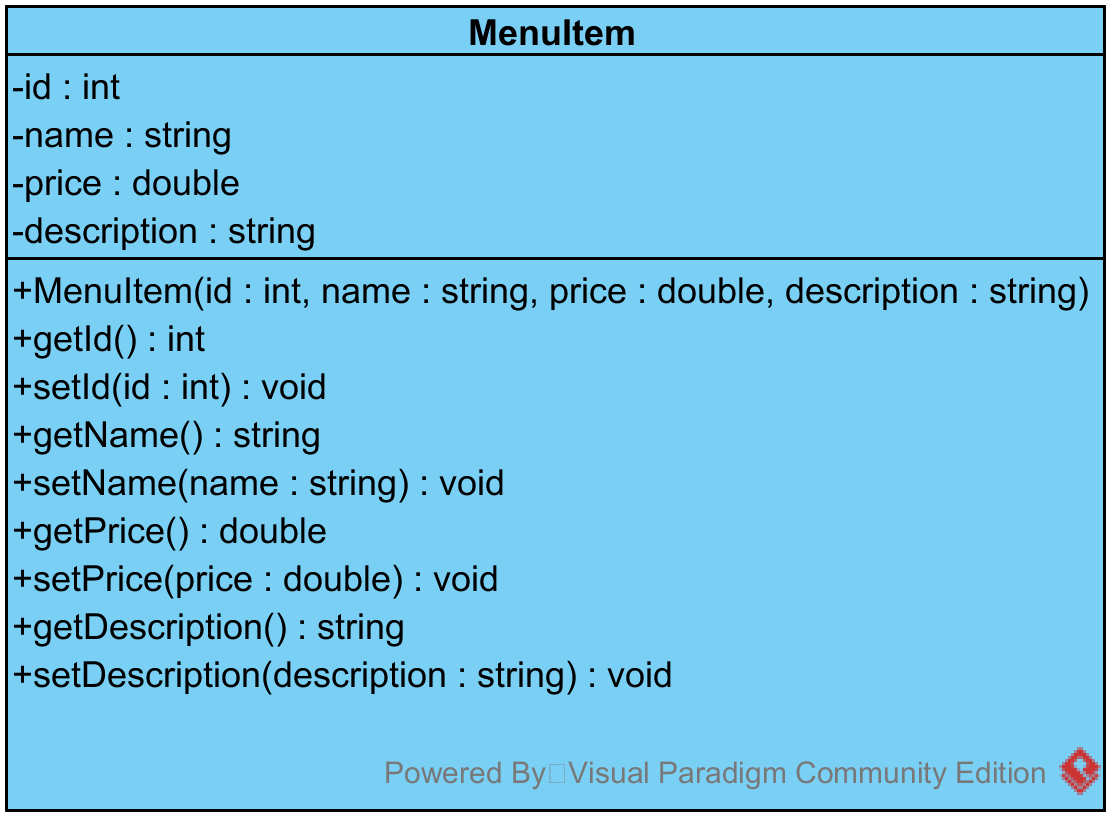
\includegraphics[width=10cm]{./diagrammi/demo/server/menuitem.png}
	\caption{Classe \class}
\end{figure}
\textbf{Descrizione:}\\
Classe che rappresenta una singola voce del menu.

\textbf{Utilizzo:}\\
Viene utilizzata per creare le singole pietanze da mostrare nel menu e da inserire negli ordini.

%\textbf{Classi ereditate:}
%\begin{itemize}
%	\item \code{}.
%\end{itemize}
%
%\textbf{Sottoclassi:}
%\begin{itemize}
%	\item \coderef{}.
%\end{itemize}

\textbf{Attributi:}
\begin{itemize}
	\item \field{- id: int}: numero identificativo della pietanza del menu;
	\item \field{- name: string}: nome della pietanza;
	\item \field{- price: double}: prezzo della pietanza;
	\item \field{- description: string}: descrizione della pietanza.
\end{itemize}

\textbf{Metodi:}
\begin{itemize}
	\item \method{+ MenuItem(id: int, name: string, price: double, description: string)}: costruttore, assegna i parametri ai corrispondenti attributi:
	\begin{itemize}
		\item \param{id: int}: id della pietanza;
		\item \param{name: string}: nome della pietanza;
		\item \param{price: double}: prezzo della pietanza;
		\item \param{description: string}: descrizione della pietanza;
	\end{itemize}
	\item \method{+ getId(): int} getter per \texttt{id};
	\item \method{+ setId(id: int): void}: setter per \texttt{id};
	\item \method{+ getName(): string} getter per \texttt{name};
	\item \method{+ setName(name: string): void}: setter per \texttt{name};
	\item \method{+ getPrice(): double} getter per \texttt{price};
	\item \method{+ setPrice(price: double): void}: setter per \texttt{price};
	\item \method{+ getDescription(): string} getter per \texttt{description};
	\item \method{+ setDesctiption(description: string): void}: setter per \texttt{description};
\end{itemize}
